\subsection{Resultados do CINTIL}
\label{resultados_cintil}
Nesta sessão, demonstraremos os resultados obtidos com a transdução do CINTIL.

\subsubsection{Treinamento} \label{result_treino_cintil}
Na Tabela \ref{tab:resultados_treino_cintil}, podemos ver o relatório de treinamento de cada execução do SP com o CINTIL transduzido.
\begin{center}
\begin{table}[h!]
    \centering
    % \begin{tabular}{c|c}
    %      &  \\
    %      & 
    % \end{tabular}
    \csvautotabular{tabelas/resultados_cintil_treino.csv}
    \caption{Resultados dos treinamentos do CINTIL, para os 10 \textit{folds}}
    \label{tab:resultados_treino_cintil}
\end{table}
\end{center}
As colunas necessitam de explicações, cuja coleta foi trabalhosa. O FAQ do SP é pouco informativo, e o do CoreNLP possui a mesma dificuldade.

Pelo código-fonte do SP\footnote{A referência foi a classe LexicalizedParser.java, que está disponível em \url{https://github.com/chbrown/stanford-parser/blob/master/edu/stanford/nlp/parser/lexparser/LexicalizedParser.java}}, \textit{States} representa a quantidade de Índices de Estado. Inferiu-se que é a quantidade de estados de transição da gramática gerada pelo treino. 

\textit{Tags}, por sua vez, representa a quantidade de Índices de \textit{Tags}. Seria a quantidade de \textit{Tags} registradas durante o treino (note que o número varia pouco).

\textit{Words}, de forma análoga, representa a quantidade de Índices de Palavras. Deduz-se que, a quantidade de palavras distintas verificadas pelo treinamento.

\textit{UnaryR} e \textit{BinaryR} correspondem, respectivamente, às quantidades de regras das gramáticas Unária e Binária. A descrição de ambas classes é, na sequencia, \textquote{\textit{Maintains efficient indexing of unary grammar rules}} e \textquote{\textit{Maintains efficient indexing of binary grammar rules}}. Pelo Javadoc do SP\footnote{\url{https://nlp.stanford.edu/nlp/javadoc/javanlp/edu/stanford/nlp/parser/lexparser/package-summary.html}},
\begin{quote}
    \begin{itemize}
        \item \textit{Unary Grammar - consists of unary rewrite rules, one per line, each of which is of the form A -> B, followed by the normalized log probability.}
        \footnote{Gramática Unária - consiste em regras de reescrita unárias, uma por linha, cada qual na forma A -> B, seguida pela probabilidade log normalizada}
        \item \textit{Binary Grammar - consists of binary rewrite rules, one per line, each of which is of the form A -> B C, followed by the normalized log probability.}
        \footnote{Gramática Binária - consiste em regras de reescrita binárias, uma por linha, cada qual na forma A -> B C, seguida pela probabilidade log normalizada}
    \end{itemize}
\end{quote}
Cabe frisar que tal modelo, utilizando regras unárias e binárias, segue o padrão da Forma Normal de Chomsky, que pode ser visto em \citeonline[p~389]{Manning1999FoundationsNLP}.

Por fim, \textit{Taggings} se refere à \textquote{\textit{[\ldots]the number of rules (tag rewrites as word) in the Lexicon.}}\footnote{o número de regras (etiquetas reescritas como palavras) no Lexicon}. Lexicon é uma interface, descrita como
\begin{quote}
    \textquote{\textit{An interface for lexicons interfacing to lexparser. Its primary responsibility is to provide a conditional probability P(word|tag), which is fulfilled by the {\#score} method. Inside the lexparser, Strings are interned and tags and words are usually represented as integers.}}
    \footnote{\textquote{Uma interface entre lexicons e o lexparser. Sua responsabilidade primária é prover uma probabilidade condicional P(palavra|etiqueta), que é preenchida pelo método \textit{\#score}. Dentro do \textit{lexparser}, \textit{Strings} são representadas canonicamente, e etiquetas e palavras são geralmente representadas por inteiros}. Tradução própria.}
\end{quote}
Pode-se notar que bons resultados de treino são obtidos apenas com o primeiro \textit{fold}, cujos resultados superam os outros \textit{folds}. Melhor visualizado na Figura \ref{fig:treino_cintil}.
\begin{center}
    \begin{figure}[!ht]
    \centering
    % \includegraphics{}
    \includesvg[width=.8\textwidth]{imagens/treino_cintil}
    % \includesvg{imagens/cintil_pcfg}
    \caption[Gráfico de resultados do treinamento, usando o CINTIL transduzido]{Gráfico de resultados do treinamento do LexicalizedParser, usando o CINTIL transduzido}
    \label{fig:treino_cintil}
\end{figure}
\end{center}

\subsubsection{Avaliação} \label{result_aval_cintil}
Nos apêndices, a Tabela \ref{tab:cintil_result_full} traz os resultados completos de nossos testes com o CINTIL. Vamos usar, aqui, versões reduzidas dos dados.

Começando pelos dados da PCFG interna ao LexicalizedParser, podemos ver o seu resultado na Tabela \ref{tab:result_cintil_pcfg}, e na Figura \ref{fig:cintil_result_pcfg}.
\begin{center}
    \begin{table}[!h]
    \centering
    \begin{tabular}{|l|c|c|c|}
        \hline
        pcfg LP/LR & LP & LR & F1\\
        \hline
        fold 1 & 58.09 & 65.99 & 61.79\\
        fold 2 & 62.52 & 62.32 & 62.42\\
        fold 3 & 55.69 & 54.58 & 55.13\\
        fold 4 & 54.03 & 51.31 & 52.63\\
        fold 5 & 61.48 & 64.64 & 63.02\\
        fold 6 & 58.81 & 57.61 & 58.21\\
        fold 7 & 62.51 & 63.67 & 63.09\\
        fold 8 & 53.03 & 54.05 & 53.54\\
        fold 9 & 61.76 & 57.5 & 59.56\\
        fold 10 & 63.32 & 63.98 & 63.65\\
        \hline
    \end{tabular}
    % \csvautotabular{resultados-cintil-testes-pcfg.csv}
    \caption{Resultados do treinamento da PCFG do SP, usando dados do CINTIL}
    \label{tab:result_cintil_pcfg}
\end{table}
        % fold 1 & 45.43 & 45.04 & 45.24\\
        % fold 2 & 42.87 & 46.27 & 44.5\\
        % fold 3 & 39.8 & 42.86 & 41.27\\
        % fold 4 & 43.55 & 47.44 & 45.42\\
        % fold 5 & 41.82 & 43.7 & 42.74\\
        % fold 6 & 41.24 & 43.26 & 42.23\\
        % fold 7 & 44.51 & 45.43 & 44.97\\
        % fold 8 & 41.61 & 44.06 & 42.8\\
        % fold 9 & 38.85 & 44.39 & 41.43\\
        % fold 10 & 39.92 & 44.13 & 41.92\\
\end{center}
Fica claro que a simples transdução de árvores da língua portuguesa para os padrões da língua inglesa, conservando as palavras, é insuficiente para o bom resultado do \textit{parser}.

Nota-se, também, que para classificações mais eficiente,s bastaria utilizar o primeiro décimo do CINTIL, pois tal bloco superou todos os outros durante o treino.
\begin{center}
    \begin{figure}[!ht]
    \centering
    % \includegraphics{}
    \includesvg[width=.8\textwidth]{imagens/cintil_pcfg}
    % \includesvg{imagens/cintil_pcfg}
    \caption[Gráfico de resultados dos testes usando o CINTIL transduzido]{Gráfico de resultados dos testes do PCFG do LexicalizedParser, usando o CINTIL transduzido}
    \label{fig:cintil_result_pcfg}
\end{figure}
\end{center}

\subsection{Estudos de caso}
\label{subsec:ec_cintil}
Separamos alguns exemplos de sentenças transduzidas, classificadas pelo \textit{Stanford Parser}. Serão exibidas as sentenças já em formato de árvore. 

O \textit{parsing} do PS é feito executando o comando \ref{lst:cod_parsing_cintil}
\begin{center}
    \begin{lstlisting}[breaklines, caption={Execução de \textit{parsing} em sentenças transduzidas a partir do CINTIL},label={lst:cod_parsing_cintil},language=Bash]
    java -cp stanford-parser.jar -mx4g edu.stanford.nlp.parser.lexparser.LexicalizedParser -loadFromSerializedFile ~/<diretorio de armazenamento>/serialGrammarBOSQUE1 sentencas_teste_cintil.txt
\end{lstlisting}
\end{center}

\begin{center}
    \begin{figure}[!ht]
    \centering
    % \includegraphics{}
    \begin{minipage}{.45\textwidth}
        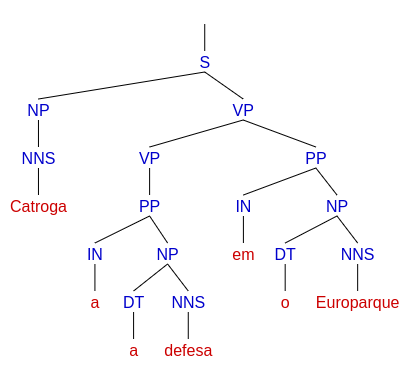
\includegraphics[width=\linewidth]{imagens/ec_cintil_sem_ponto_tree_trans.png}
        % \begin{forest}
        %     [
        %      [S 
        %       [NP 
        %       [NNS Catroga]
        %       ]
        %       [VP 
        %       [VP 
        %         [PP 
        %          [\textbf{IN a\_}]
        %          [NP 
        %           [\textbf{DT a}]
        %           [NNS defesa]
        %          ]
        %         ]
        %       ]
        %       [PP 
        %         [\textbf{IN em\_}]
        %         [NP 
        %          [\textbf{DT o}]
        %          [NNS Europarque]
        %         ]
        %       ]
        %       ]
        %      ]
        %     ]
        % \end{forest}
    \end{minipage}
    % 
    \begin{minipage}{.45\textwidth}
        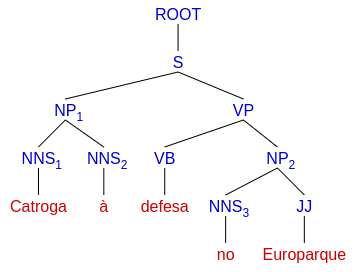
\includegraphics[width=\linewidth]{imagens/ec_cintil_sem_ponto_tree_sp.png}
        % \begin{forest}
        %     [ROOT
        %       [S
        %         [NP [NNS Catroga] [\textbf{JJ à}]]
        %         [VP [VB defesa]
        %           [NP [\textbf{NNS no}] [JJ Europarque]]]]]
        % \end{forest}
    \end{minipage}
    \caption[Estudo de caso CINTIL - Sentença transduzida sem pontuação]{Estudo da sentença eCTMP-000647/78121, \textquote{Catroga à defesa no Europarque}, que originalmente não possui nenhuma pontuação}
    \label{fig:ec_cintil_sem_ponto_tree}
\end{figure}
\end{center}
Na Figura \ref{fig:ec_cintil_sem_ponto_tree}, vemos o resultado da classificação de uma sentença originalmente sem pontuações. Há algumas coisas interessantes a serem notadas. Se, por um lado, de fato a falta de pontuação ajudou no \textit{parsing}, por outro o SP tem dificuldades em separar contrações de preposições.
% (nós marcados em negrito).
\begin{center}
    \begin{figure}[!ht]
    \centering
    a)
    \begin{minipage}{.45\textwidth}
        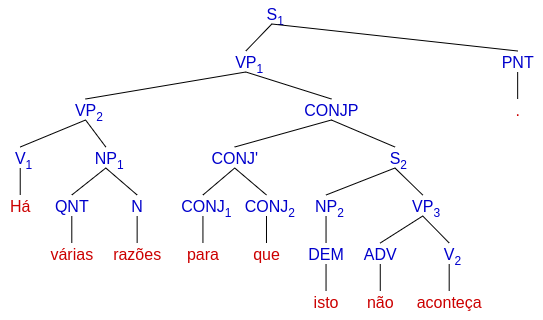
\includegraphics[width=\linewidth]{imagens/ec_cintil_conjp_tree_orig.png}
    \end{minipage}
    \hfill
    b)
    \begin{minipage}{.45\textwidth}
        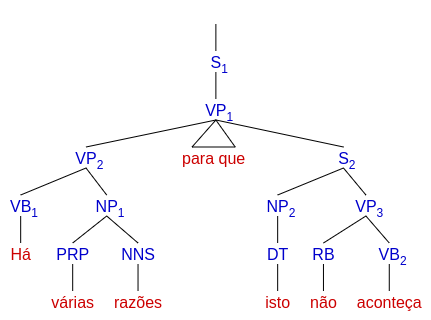
\includegraphics[width=\linewidth]{imagens/ec_cintil_conjp_tree_trans.png}
    \end{minipage}
    \hfill
    \vskip\floatsep
    c)
    \begin{minipage}{.45\textwidth}
        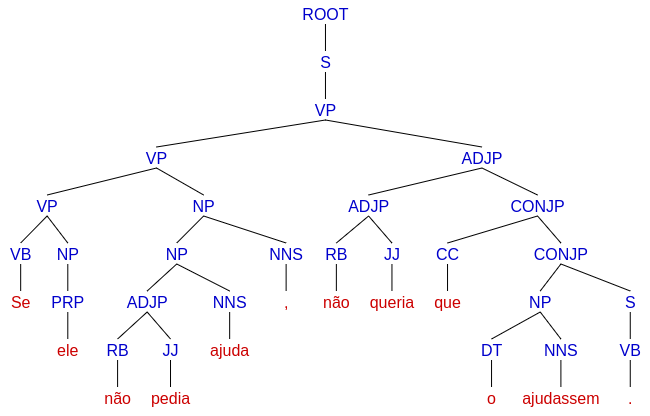
\includegraphics[width=\linewidth]{imagens/ec_cintil_conjp_tree_sp.png}
    \end{minipage}
    \caption[Estudo de caso CINTIL - Árvore da sentença transduzida com CONJP]{Estudo da sentença eCTMP-001150/117736, \textquote{Há várias razões para que isto não aconteça.}, que possui CONJP internamente. Em a), temos a árvore como se apresenta originalmente no CINTIL. Em b), temos a mesma sentença, pós transdução. Em c), temos o resultado da classificação do SP, utilizando a gramática gerada neste trabalho (após o processo de transdução)}
    \label{fig:ec_cintil_conjp_tree}
\end{figure}
\end{center}
A Figura \ref{fig:ec_cintil_conjp_tree} nos dá mais material de interesse. Por exemplo, pode-se notar como a ausência de conhecimento de léxico da língua classificada gera confusões. O \textquote{o} é facilmente confundido, mas não apenas. A adjunção de CONJP, que existe no CINTIL unicamente para o posicionamento do PNT, aparentemente confunde o SP, que a transforma num adjunto de VP. O sintagma VP, em \textquote{não podia} tem seu núcleo, e por conseguinte, o sintagma como um todo, alterado. Provavelmente, para seguir a tendência da língua inglesa, que costuma ter o núcleo do sintagma posicionado mais à direita \citeonline[p~40]{charniak97statistical}. A confusão com as pontuações é notável, sendo transformadas em substantivo (NNS) ou verbo (VB), o que é curioso. Supões-se que o SP não seja estranho à pontuações mesmo que elas não venham no seu conjunto de treino.
\begin{center}
    \begin{figure}[!ht]
    \centering
    \begin{minipage}{.45\textwidth}
        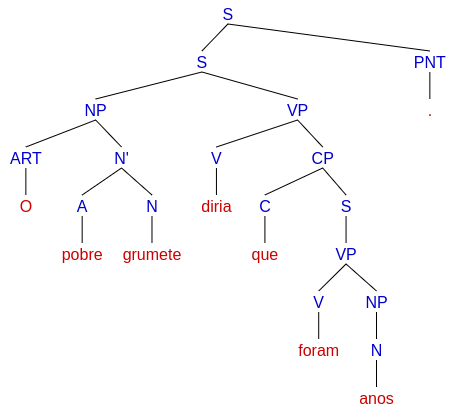
\includegraphics[width=\linewidth]{imagens/ec_cintil_cp_tree_orig.png}
        \caption{árvore original}
    \end{minipage}
    \hfill
    \begin{minipage}{.45\textwidth}
        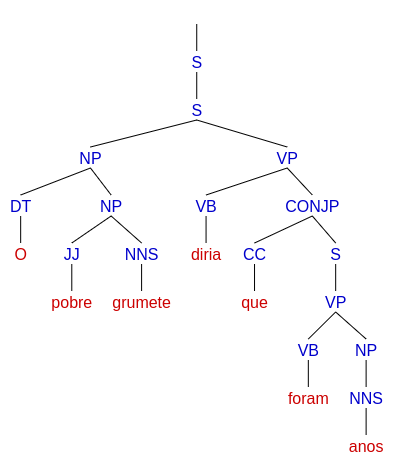
\includegraphics[width=\linewidth]{imagens/ec_cintil_cp_tree_trans.png}
        \caption{árvore transduzida}
    \end{minipage}
    \hfill
    \vskip\floatsep
    \begin{minipage}{.45\textwidth}
        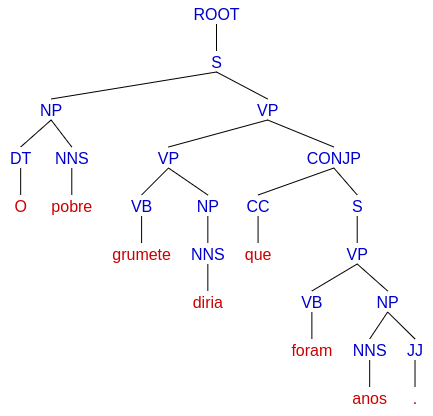
\includegraphics[width=\linewidth]{imagens/ec_cintil_cp_tree_sp.png}
        \caption{árvore gerada pelo SP}
    \end{minipage}
    \caption[Estudo de caso CINTIL - Árvore da sentença transduzida com CP]{Estudo da sentença eCTMP-000694/81773, \textquote{O pobre grumete diria que foram anos.}, que possui CP internamente.}
    \label{fig:ec_cintil_cp_tree}
\end{figure}
\end{center}
Sobre o sintagma CP, a Figura \ref{fig:ec_cintil_cp_tree}. Curiosamente, o sintagma em questão está acompanhando bem a estrutura da árvore original, e da árvore transduzida. O maior destaque ficam para as palavras de classe aberta (substantivos, verbos, adjetivos). Aparentemente, a informação léxica continua sendo um problema.
\begin{center}
    \begin{figure}[!ht]
    \centering
    \begin{minipage}{.45\textwidth}
        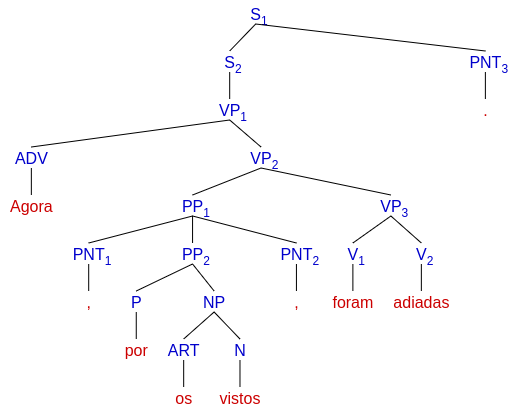
\includegraphics[width=\linewidth]{imagens/ec_cintil_virgula_tree_orig.png}
        \caption{árvore original}
    \end{minipage}
    \hfill
    \begin{minipage}{.45\textwidth}
        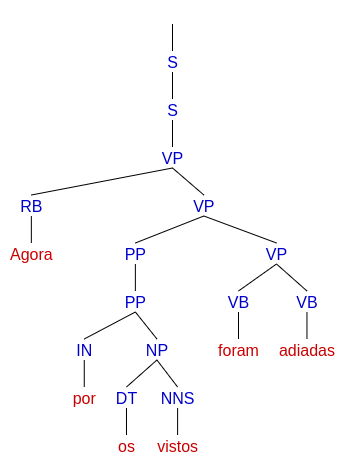
\includegraphics[width=\linewidth]{imagens/ec_cintil_virgula_tree_trans.png}
        \caption{árvore transduzida}
    \end{minipage}
    \hfill
    \vskip\floatsep
    \begin{minipage}{.45\textwidth}
        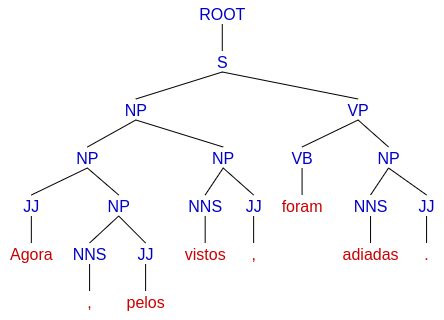
\includegraphics[width=\linewidth]{imagens/ec_cintil_virgula_tree_sp.png}
        \caption{árvore gerada pelo SP}
    \end{minipage}
    \caption[Estudo de caso CINTIL - Árvore da sentença transduzida com vírgulas]{Estudo da sentença eCTMP-001597/153293, \textquote{Agora, pelos vistos, foram adiadas.}, que possui vírgulas.}
    \label{fig:ec_cintil_virgula_tree}
\end{figure}
\end{center}
Por fim, para finalizar nossa revisão com as transduções do CINTIL, temos a Figura \ref{fig:ec_cintil_virgula_tree}. Nota-se uma tendência muito interessante, do SP, de considerar palavras como adjetivo (JJ). Mesmo para palavras que nunca assumem tal forma, como \textquote{pelos}, que pode ser ou a contração \textit{por + os}, ou um substantivo. A falta de treinamento com pontuações mais uma vez é sentida, uma vez que SP não sabe como resolver vírgulas e pontos.